\section{Multi-Task and Meta Learning}\label{sec:multi-meta}

To study how we can enable agents to learn skills in the real world, let's consider robots: they can teach us things about intelligence, because they faced with the real world , they must generalize across tasks, objects and environments, they need some common sense understanding, they can't rely on supervision. Nowadays, robots/agents can learn very well a single task in a single environment, starting from scratch, relying on detailed supervision and guidance, moreover, often the researcher has to do lot of work to train the robot.

Deep learning allows us to handle unstructured inputs (pixels, language...) without hand engineering features, with less domain knowledge, but we need huge diverse data to generalize. For some tasks, by the way, we don't have large datasets, in other cases it is impractical to learn from scratch for each specific task, in still other cases, the dataset is unbalanced (\textit{long tail}: few classes with lots of data-points), moreover, sometimes we need to quickly learn something new. In all these cases, standard ML paradigms don't work.

Multi-task learning and meta-learning can overcome these problems. A \textit{task} is identified by a dataset, a loss function, and a parameterized model $f_\theta$. To apply these strategies, we need that the tasks we consider share some structure, but this is often the case.

Informal problem definitions:
\begin{myitem}
    \item \textbf{The multi-task learning problem}: Learn all of the tasks more quickly or more proficiently than learning them independently.
    \item \textbf{The meta-learning problem}: Given data/experience on previous tasks, learn a new task more quickly and/or more proficiently.
\end{myitem}

Furthermore, multi-task and meta-learning are critical for the \textit{democratization} of AI: research datasets are huge, while real-world datasets are much smaller.


\subsection{Multi-Task Learning}\label{sec:mm-multi}

Multi-task learning can reduce to single task learning, by aggregating the data across tasks and learning a single model, but we can do better if we exploit the fact that we know that data is coming from different tasks.

Formally, in single-task supervised learning a task is defined by the dataset $\mathcal{D} = \left\{(x,y)_k\right\}$ and the objective $\min_\theta \mathcal{L}(\theta, \mathcal{D})$, where usually the loss is negative log likelihood $\mathcal{L}(\theta, \mathcal{D}) = - \mathbb{E}_{(x,y)\sim\mathcal{D}} \left[\log_{f_\theta}(y|x)\right]$. On the other hand, a task in a multi-task learning context is defined as a data generating distribution $\mathcal{T}_i := \left\{ p_i(x), p_i (y|x), \mathcal{L}_i \right\}$, with corresponding datasets $\mathcal{D}_i^{tr}$ and $\mathcal{D}_i^{test}$. Example of multi-task learning are:
\begin{myitem}
    \item \textit{multi-task classification}, such as per-language handwriting recognition, where $\mathcal{L}_i$ is the same across all tasks;
    \item \textit{multi-label learning}, such as scene understanding, where $\mathcal{L}_i$ and $p_i(x)$ are the same across all tasks.
\end{myitem}
When you care more about one task than another, also $\mathcal{L}_i$ varies.

We can add a parameter $z_i$ to represent the \textit{task descriptor} (for example with the task index), so that the function learned by the model is $f_\theta(y|x,z_i)$ instead of $f_\theta(y|x)$. Now we must find a way to optimize the objective
\begin{equation}\label{eq:multi-task-objective}
    \min_\theta \sum_{i=1}^{T} \mathcal{L}_i (\theta, \mathcal{D}_i).
\end{equation}

In other words, we have to find a way to condition on $z_i$, in order to share as little as possible. A solution is independent training within a single network, with no shared parameters, and multiplicative gating to compute the output: $y = \sum_j \mathbbm{1}(z_i = j) y_j$ (see figure \ref{fig:mm-multitask-sol1}). The opposite solution is to concatenate $z_i$ with input and/or activations, so that all parameters are shared, except those directly following $z_i$ (see figure \ref{fig:mm-multitask-sol2}).

\begin{minipage}{.5\linewidth}
    \begin{figure}[H]
        \centering
        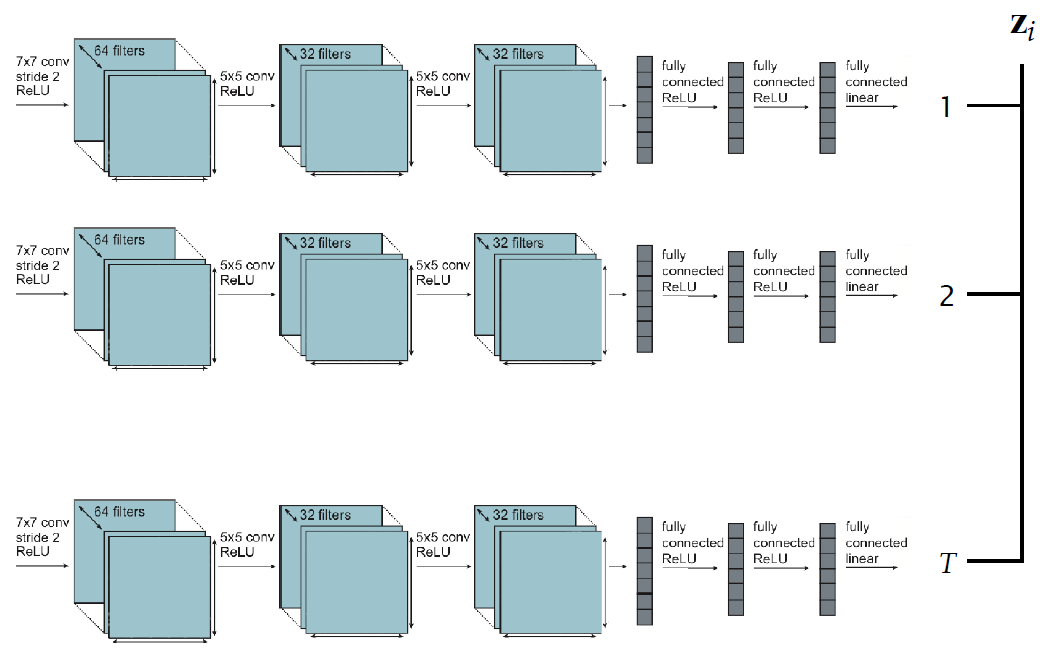
\includegraphics[width=.95\linewidth]{images/mm-multitask-sol1}
        \caption[Solution 1]{Solution 1}
        \label{fig:mm-multitask-sol1}
    \end{figure}
\end{minipage}
\begin{minipage}{.5\linewidth}
    \begin{figure}[H]
        \centering
        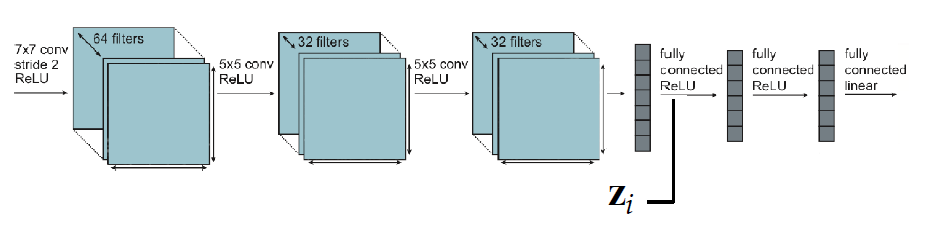
\includegraphics[width=.95\linewidth]{images/mm-multitask-sol2}
        \caption[Solution 2]{Solution 2}
        \label{fig:mm-multitask-sol2}
    \end{figure}
\end{minipage}

An alternative view on the multi-task objective is to split the parameter $\theta$ into shared parameters $\theta^{sh}$ and task specific parameters $\theta^i$. Then, our objective becomes
\begin{equation}\label{eq:multi-task-objective-2}
    \min_{\theta^{sh}, \theta^1, \ldots, \theta^T} \sum_{i=1}^{T} \mathcal{L}_i \left(\left\{ \theta^{sh}, \theta^i \right\}, \mathcal{D}_i \right).
\end{equation}
In this way, choosing how to condition on $z_i$ is equivalent to choosing how and where to share parameters:
\begin{myenum}
    \item Concatenation-based conditioning (see figure \ref{fig:mm-multitask-sol3});
    \item Additive conditioning (see figure \ref{fig:mm-multitask-sol4});
    \item Multi-head architecture (see figure \ref{fig:mm-multitask-sol6});
    \item Multiplicative conditioning (see figure \ref{fig:mm-multitask-sol7}), good because more expressive, and able to generalize independent networks and independent heads.
\end{myenum}
Notice that solutions 1 and 2 are equivalent, as shown in figure \ref{fig:mm-multitask-sol5}.\\
Unfortunately, these design decisions are like neural network architecture tuning: problem dependent and largely guided by intuition or knowledge of the problem.

\begin{minipage}{.33\linewidth}
    \begin{figure}[H]
        \centering
        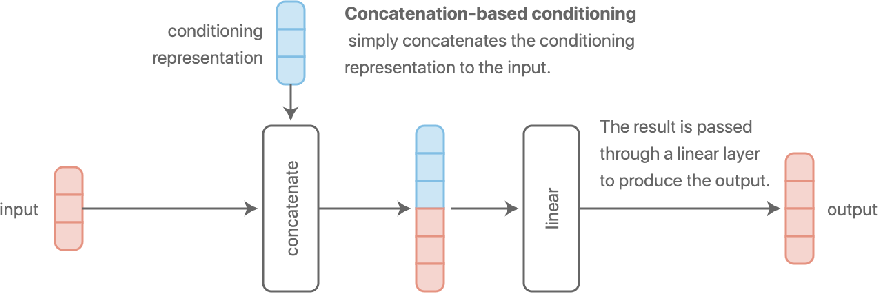
\includegraphics[width=0.95\linewidth]{images/mm-multitask-sol3}
        \caption[Concatenation-based conditioning]{Concatenation-based conditioning}
        \label{fig:mm-multitask-sol3}
    \end{figure}
\end{minipage}
\begin{minipage}{.33\linewidth}
    \begin{figure}[H]
        \centering
        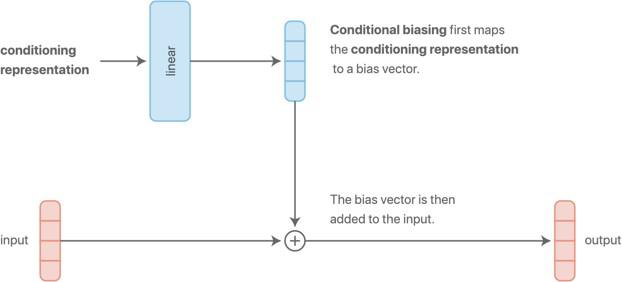
\includegraphics[width=0.95\linewidth]{images/mm-multitask-sol4}
        \caption[Additive conditioning]{Additive conditioning}
        \label{fig:mm-multitask-sol4}
    \end{figure}
\end{minipage}
\begin{minipage}{.33\linewidth}
    \begin{figure}[H]
        \centering
        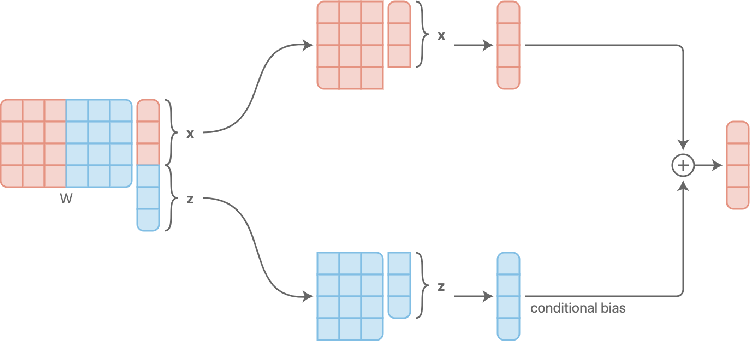
\includegraphics[width=0.95\linewidth]{images/mm-multitask-sol5}
        \caption[Concatenation $\equiv$ Additive]{Concatenation $\equiv$ Additive}
        \label{fig:mm-multitask-sol5}
    \end{figure}
\end{minipage}

\begin{minipage}{.4\linewidth}
    \begin{figure}[H]
        \centering
        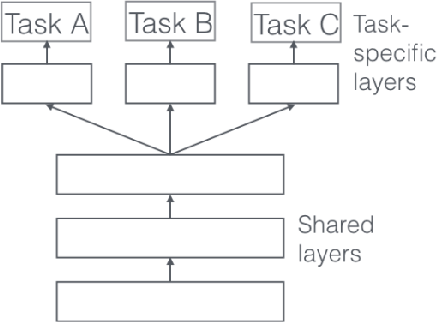
\includegraphics[width=0.7\linewidth]{images/mm-multitask-sol6}
        \caption[Multi-head architecture]{Multi-head architecture}
        \label{fig:mm-multitask-sol6}
    \end{figure}
\end{minipage}
\begin{minipage}{.6\linewidth}
    \begin{figure}[H]
        \centering
        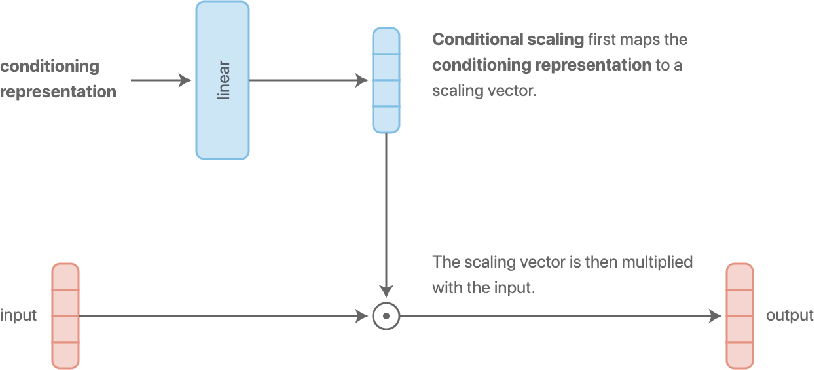
\includegraphics[width=0.8\linewidth]{images/mm-multitask-sol7}
        \caption[Multiplicative conditioning]{Multiplicative conditioning}
        \label{fig:mm-multitask-sol7}
    \end{figure}
\end{minipage}

To optimize the objective in equation \ref{eq:multi-task-objective}, we have to follow the steps below:
\begin{myenum}
    \item Sample mini-batch of tasks $\mathcal{B} \sim \left\{\mathcal{T}_i\right\}$;
    \item Sample mini-batch datapoints for each task $\mathcal{D}_i^b \sim \mathcal{D}_i$;
    \item Compute loss on the mini-batch $\hat{\mathcal{L}}(\theta, \mathcal{B}) = \sum_{\mathcal{T}_k \in \mathcal{B}} \mathcal{L}_k (\theta, \mathcal{D}_k^b)$;
    \item Backpropagate loss to compute gradient $\nabla_\theta \hat{\mathcal{L}}$;
    \item Apply gradient with a neural network optimizer.
\end{myenum}
This approach ensures that tasks are sampled uniformly, regardless of data quantities. For regression problems, we must make sure that task labels are on the same scale.

Two main problems may arise in multi-task learning. The first one is \textit{negative transfer}: sometimes independent networks work the best. This may happen for different reasons: optimization challenges caused by cross-task interference or tasks that learn at different rates, or by limited representational capacity (multi task networks often need to be much larger than their single task counterparts). The solution is to share less across tasks (i.e., \textit{soft parameter sharing}):
\begin{equation}\label{eq:multi-task-objective-3}
    \min_{\theta^{sh}, \theta^1, \ldots, \theta^T} \sum_{i=1}^{T} \mathcal{L}_i \left(\left\{ \theta^{sh}, \theta^i \right\}, \mathcal{D}_i \right) + \sum_{t'=1}^{T} \norm{\theta^t - \theta^{t'}}.
\end{equation}
This allows for more fluid degrees of parameter sharing, but adds more design decisions.\\
The second problem is overfitting. It may be due to too little sharing among tasks. In this sense, we can look at multi-task learning as a form of regularization. The solution is to share more.


\subsection{Meta-Learning}\label{sec:mm-meta}

We would like for the machines to be able to understand, generalize and learn from few similar - not identical - examples as human are, but they aren't, even though they are getting better at it, for example with \textit{human-level concept learning through probabilistic program induction}.

The main problem we have to deal with in this case, is \textbf{few-shot learning}: we want to design a learning algorithm $A$ that outputs good parameters $\theta$ of a model $M$, when fed a small dataset $\mathcal{D}^{tr} = \left\{x_i, y_i\right\}_{i=1}^L$. The idea is to learn $A$ end-to-end. This approach is called \textit{meta-learning}, or \textit{learning to learn}.

Related works are:
\begin{myitem}
    \item \textit{Transfer learning}: large image datasets have been shown to allow training representations that transfer to other problems, while, in few shot learning, we aim at transferring the complete training of the model on new datasets (not just transferring the features or initialization), and ideally there should be no human involved in producing a model for new datasets;
    \item \textit{One-shot learning}: old studies largely relied on hand-engineered features, but with recent progress in end-to-end deep learning, we hope to learn a representation better     suited for few-shot learning;
    \item \textit{Neural Architecture Search}: techniques based on Bayesian optimization and reinforcement learning to look for the best NN hyperparameters.
\end{myitem}
But, if you don't evaluate on never-seen problems/datasets, it's not meta-learning.

Let's define a learning algorithm $A$ as:
\begin{myitem}
    \item \textit{input}: training set $\mathcal{D}^{\text{tr}} = {(x_i, y_i)}$,
    \item \textit{output}: parameters $\theta$ for the model $M$ (the \textit{learner}),
    \item \textit{objective}: good performance on the test set $\mathcal{D}^{\text{test}} = {(x'_i, y'_i)}$;
\end{myitem}
then, a meta-learning algorithm can be defined as:
\begin{myitem}
    \item \textit{input}: meta-training set $\mathcal{D}^{\text{meta-train}} = \left\{\left(D_{\text{train}}^{(n)}, D_{\text{test}}^{(n)}\right)\right\}_{n=1}
    ^N$ of episodes,
    \item \textit{output}: parameters $\theta$ of an algorithm $A$ (the \textit{meta-learner}), to learn model $M$,
    \item \textit{objective}: good performance on the meta-test set $\mathcal{D}^{\text{meta-test}} = \left\{\left({D'}_{\text{train}}^{(n)}, {D'}_{\text{test}}^{(n)}\right)\right\}_{n=1}^{N'}$.
\end{myitem}
Thus, a couple of (training set, test set), that are used to train a \textit{learner}, is an \textit{episode}, and a set of episodes composes a meta-training set, which is used to train a \textit{meta-learner}.
Someone calls the training set ``support set'' and the test set ``query set'', in this case, the meta-training set and the meta-test set can be called simply training test and test set, respectively.
The approach is shown in figure \ref{fig:mm-meta-learning}.

\begin{figure}[h!]
    \centering
    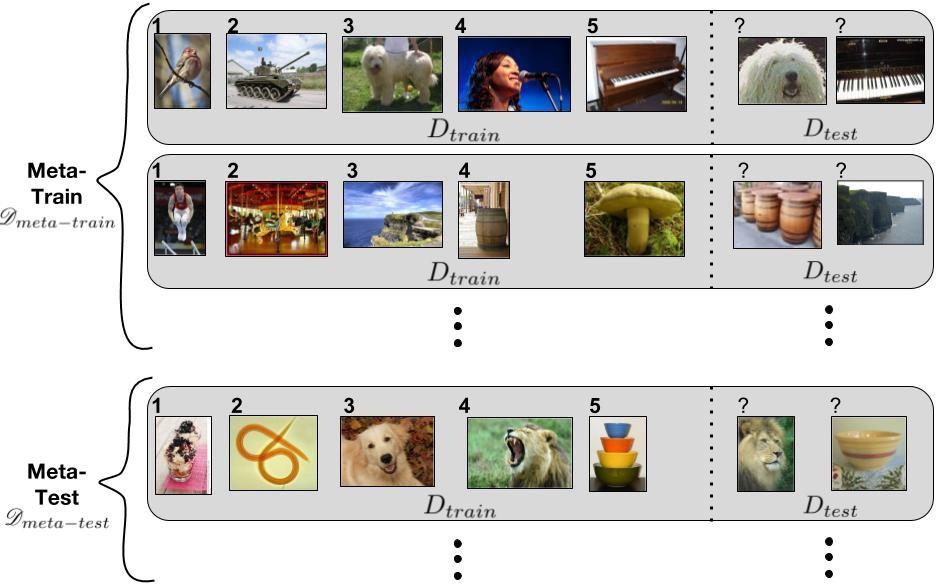
\includegraphics[width=0.6\linewidth]{images/mm-meta-learning}
    \caption[Meta-learning]{Meta-learning}
    \label{fig:mm-meta-learning}
\end{figure}

To evaluate few-shot image recognition, a useful dataset is \textit{Omniglot}, a transpose of MNIST for meta-learning tasks, with many classes and few examples, from 50 different alphabets. Other datasets used for this task are \textit{MiniImagenet, CIFAR, CUB, CelebA}. A possible evaluation strategy is \textit{5-way, 1-shot image classification}: given 1 example of 5 classes, classify new examples.


\subsubsection{Optimization-based Techniques}\label{sec:mm-optimization}

The key idea is to acquire $\phi_i$ through optimization of
\begin{equation}\label{eq:meta-learn-optimization}
    \max_{\phi_i} \log p(\mathcal{D}_i^{tr} | \phi_i) + \log p(\phi_i | \theta).
\end{equation}
The meta-parameters $\theta$ serve as a prior, e.g.: initialization for \textit{fine-tuning}. In this case, for many gradient steps, during training we fine-tune in this way:
\begin{equation}\label{eq:meta-learn-fine-tuning}
    \phi \gets \theta - \alpha \nabla_\theta \mathcal{L}(\theta, \mathcal{D}^{tr}),
\end{equation}
where $\theta$ are pre-trained parameters from a similar task with a big datasets and $\mathcal{D}^{tr}$ training data for the new task.

Some common practices:
\begin{myitem}
    \item Fine tune with a smaller learning rate;
    \item Lower learning rate for lower layers;
    \item Freeze earlier layers, gradually unfreeze;
    \item Reinitialize last layer;
    \item Search over hyperparameters via cross validation;
    \item Architecture choices matter.
\end{myitem}
Notice that fine-tuning is less effective with very small datasets.

At test time, apply meta-learning by optimizing this objective:
\begin{equation}\label{eq:meta-learn-objective}
    \min_\theta \sum_{\text{task } i} \mathcal{L} \left( \theta - \alpha \nabla_\theta \mathcal{L}(\theta, \mathcal{D}_i^{tr}), \mathcal{D}_i^{test} \right)
\end{equation}
where $\theta$ is the parameter vector being meta-learned.
The key idea is to learn parameter vector $\theta$ that transfers via fine tuning, over many tasks (see figure \ref{fig:mm-meta-learning1}, where $\phi_i^*$ is the optimal parameter vector for task $i$).

\begin{figure}[h!]
    \centering
    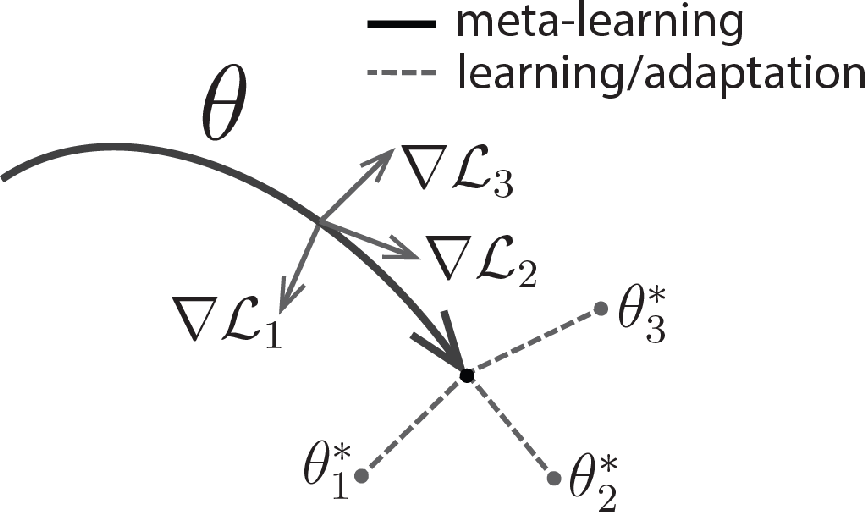
\includegraphics[width=0.4\linewidth]{images/mm-meta-learning1}
    \caption[Optimization-Based Inference]{Optimization-Based Inference}
    \label{fig:mm-meta-learning1}
\end{figure}

Thus, the optimization-based approach works like this:
\begin{myenum}
    \item Sample task $\mathcal{T}_i$ (or mini batch of tasks);
    \item Sample disjoint datasets $\mathcal{D}_i^{tr}, \mathcal{D}_i^{test}$ from $\mathcal{D}_i$;
    \item Optimize equation \ref{eq:meta-learn-fine-tuning};
    \item Update $\theta$ using $\nabla_\theta \mathcal{L}\left(\phi_i, \mathcal{D}_i^{test} \right)$;
    \item Restart from step 1.
\end{myenum}
This brings up second-order derivatives (the Hessian), which isn't explicitly computed. No higher order derivatives are needed for more gradient descent steps.


\subsubsection{Non-parametric Techniques}\label{sec:mm-non-parametric}

The key idea is to use a \textit{non-parametric learner}: given a training set $\mathcal{D}_i^{tr}$ and a test data-point $x^{test}$, compare test image with training images. Pixel space or L2 distance aren't appropriate, so we learn to compare using meta-training data: train a Siamese network to predict whether two images belong to the same class (meta-training with binary classification), then test comparing image $x^{test}$ to each image in $\mathcal{D}_j^{tr}$ (meta-test with $N$-way classification).

It is possible to combine meta-train and meta-test in a unique network trained end-to-end in order to find nearest neighbors in the learned embedding space (see figure \ref{fig:mm-meta-learning2}). The network output is $\hat{y} = \sum_{i=1}^{k} a(\hat{x}, x_i)y_i$, where $a(\hat{x}, x_i) = \frac{e^{c(f(\hat{x}), g(x_i))}}{\sum_{j=1}^k e^{c(f(\hat{x}), g(x_j))}}$.

\begin{figure}[h!]
    \centering
    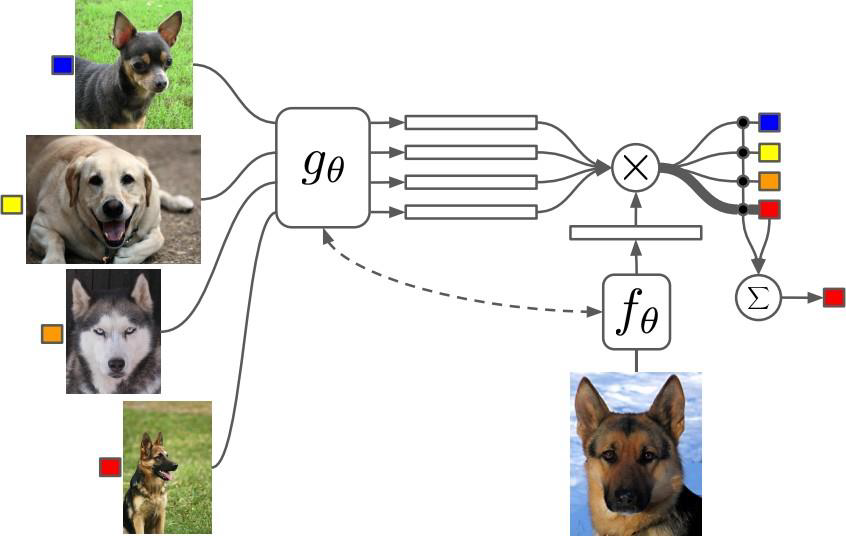
\includegraphics[width=0.7\linewidth]{images/mm-meta-learning2}
    \caption[Matching Networks]{Matching Networks}
    \label{fig:mm-meta-learning2}
\end{figure}

An alternative is to train a \textbf{prototype extractor} (see figure \ref{fig:mm-meta-learning3}):
\begin{flalign}\label{eq:meta-learn-prototype}
    p_\phi(y=k|x) &= \frac{\exp(-d(f_\phi(x), c_k))}{\sum_{k'}\exp(-d(f_\phi(x), c_{k'})}\\
    d &= \text{Euclidean or Cosine distance}\\
    c_k &= \frac{1}{\abs{S_k}} \sum_{(x_i, y_i) \in S_k} f_\phi (x_i)\\
    S_k &= \left\{ (x_i, y_i) | y_i = k, (x_i, y_i) \in \mathcal{D}^{tr} \right\}\\
    \phi &\equiv \Theta
\end{flalign}

\begin{figure}[h!]
    \centering
    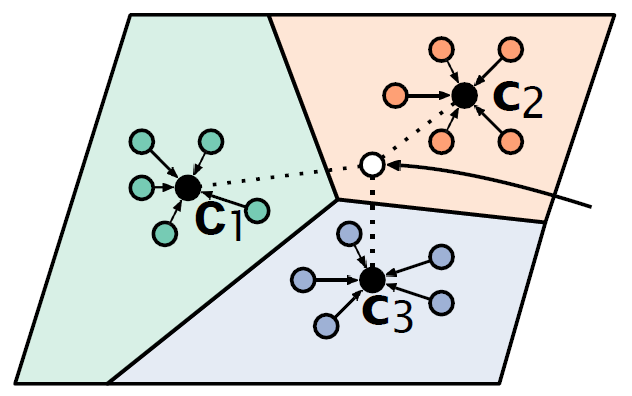
\includegraphics[width=0.5\linewidth]{images/mm-meta-learning3}
    \caption[Prototypical Networks]{Prototypical Networks}
    \label{fig:mm-meta-learning3}
\end{figure}
